% !TEX TS-program = pdflatex
% !TEX encoding = UTF-8 Unicode

% This is a simple template for a LaTeX document using the "article" class.
% See "book", "report", "letter" for other types of document.

\documentclass[12pt]{article} % use larger type; default would be 10pt
\usepackage[fontsize=12pt]{fontsize}
\renewcommand{\baselinestretch}{1.5} % linespacing=1.5
\usepackage[T2A]{fontenc} % кодировка
\usepackage{fontspec} % for changing fonts 
% \setmainfont{Times New Roman}
\setmainfont{Minion Pro}
% \setmainfont{Roboto}
% \usepackage[utf8]{inputenc} % set input encoding (not needed with XeLaTeX)
\usepackage[english]{babel} % for cyrillic letters support
\usepackage[parfill]{parskip} % remove space vefore parapraph
\setlength{\parskip}{0pt} % additional skip between paragraphs


%%% PAGE DIMENSIONS
\usepackage{geometry} % to change the page dimensions
\geometry{a4paper} % or letterpaper (US) or a5paper or....
\geometry{left=30mm,right=20mm,top=15mm, bottom=15mm} % for example, change the margins to 2 inches all round
% \graphicspath{{./images/}}
% \geometry{landscape} % set up the page for landscape
%   read geometry.pdf for detailed page layout information

\usepackage{graphicx} % support the \includegraphics command and options

% \usepackage[parfill]{parskip} % Activate to begin paragraphs with an empty line rather than an indent

%%% PACKAGES
\usepackage{blindtext}
\usepackage{booktabs} % for much better looking tables
\usepackage{multirow}
\usepackage{array} % for better arrays (eg matrices) in maths
\usepackage{paralist} % very flexible & customisable lists (eg. enumerate/itemize, etc.)
\usepackage{verbatim} % adds environment for commenting out blocks of text & for better verbatim
\usepackage{subfig} % make it possible to include more than one captioned figure/table in a single float
\usepackage{cmap} % search in pdf
\usepackage{longtable} % for long tables 
\usepackage{lscape}
\usepackage{hyperref} % for hyperlinks
\usepackage{listings} % for code listings
% These packages are all incorporated in the memoir class to one degree or another...

%% Useful packages
\usepackage[colorinlistoftodos]{todonotes}
% \usepackage[colorlinks=true, allcolors=blue]{hyperref}



\usepackage{amsmath,amsthm,amsfonts,amssymb,amscd, fancyhdr, color, comment, graphicx, environ}
\usepackage{float}
\usepackage{mathrsfs}
\usepackage[math-style=ISO]{unicode-math}
\setmathfont{TeX Gyre Termes Math}
\setmonofont{Hack Nerd Font Mono}
\usepackage{lastpage}
\usepackage[dvipsnames]{xcolor}
% \usepackage[framemethod=TikZ]{mdframed}
\usepackage{indentfirst}
\usepackage{thmtools}
\usepackage{shadethm}
\usepackage{setspace}


\definecolor{codegreen}{rgb}{0,0.6,0}
\definecolor{codegray}{rgb}{0.5,0.5,0.5}
\definecolor{codepurple}{rgb}{0.58,0,0.82}
\definecolor{backcolour}{rgb}{0.95,0.95,0.92}


%%% HEADERS & FOOTERS
\usepackage{fancyhdr} % This should be set AFTER setting up the page geometry
\pagestyle{fancy} % options: empty , plain , fancy
\renewcommand{\headrulewidth}{0pt} % customise the layout...
\lhead{}\chead{}\rhead{}
\lfoot{}\cfoot{\thepage}\rfoot{}

%%% SECTION TITLE APPEARANCE
\usepackage{titlesec}
\usepackage{sectsty}
\sectionfont{\centering}
\subsectionfont{\centering}

\usepackage{enumitem}
\setlist{nolistsep}

\hypersetup{
    colorlinks=true,
    linkcolor=black,
    filecolor=magenta,      
    urlcolor=blue,
    pdftitle={Overleaf Example},
    pdfpagemode=FullScreen,
    }
\urlstyle{same}




\lstdefinestyle{mystyle}{
    extendedchars=\true,
    inputencoding=utf8x,
    backgroundcolor=\color{backcolour},   
    commentstyle=\color{codegreen},
    keywordstyle=\color{magenta},
    numberstyle=\tiny\color{codegray},
    stringstyle=\color{codepurple},
    basicstyle=\ttfamily\footnotesize,
    breakatwhitespace=false,         
    breaklines=true,                 
    captionpos=b,                    
    keepspaces=true,                 
    numbers=left,                    
    numbersep=5pt,                  
    showspaces=false,                
    showstringspaces=false,
    showtabs=false,                  
    tabsize=2
}

\lstset{style=mystyle}




% \allsectionsfont{\sffamily\mdseries\upshape} % (See the fntguide.pdf for font help)
% (This matches ConTeXt defaults)

%%% ToC (table of contents) APPEARANCE
% \usepackage[nottoc,notlof,notlot]{tocbibind} % Put the bibliography in the ToC
% \usepackage[titles,subfigure]{tocloft} % Alter the style of the Table of Contents
% \renewcommand{\cftsecfont}{\rmfamily\mdseries\upshape}
% \renewcommand{\cftsecpagefont}{\rmfamily\mdseries\upshape} % No bold!
\makeatletter
\renewcommand{\fnum@figure}{Picture. \thefigure}
\makeatother



\renewcommand\lstlistingname{Algorithm}
\renewcommand\lstlistlistingname{Algorithms}
\def\lstlistingautorefname{Alg.}


\title{Графовые алгоритмы и структуры данных}
\author{Бактыбеков Н.Б.}

\begin{document}
\begin{titlepage}

\newcommand{\HRule}{\rule{\linewidth}{0.5mm}} % Defines a new command for the horizontal lines, change thickness here

%----------------------------------------------------------------------------------------
%	LOGO SECTION
%----------------------------------------------------------------------------------------
\centering

\includegraphics[width=8cm]{title/logo_inai.jpg}\\[1cm] % Include a department/university logo - this will require the graphicx package
 
%----------------------------------------------------------------------------------------

\center % Center everything on the page

%----------------------------------------------------------------------------------------
%	HEADING SECTIONS
%----------------------------------------------------------------------------------------

\textsc{\LARGE СРСП №3}\\[1.5cm] 
\textsc{\Large }\\[0.5cm] 
\textsc{\large WIN-1-22}\\[0.5cm] 

%----------------------------------------------------------------------------------------
%	TITLE SECTION
%----------------------------------------------------------------------------------------
\makeatletter
\HRule \\[0.4cm]
{ \huge \bfseries \@title}\\[0.4cm] % Title of your document
\HRule \\[6.5cm]
 
%----------------------------------------------------------------------------------------
%	AUTHOR SECTION
%----------------------------------------------------------------------------------------

\begin{minipage}{0.4\textwidth}
\begin{flushleft} \large
\emph{Выполнил:}\\
\@author % Your name



\end{flushleft}
\end{minipage}
~
\begin{minipage}{0.4\textwidth}
\begin{flushright} \large
\emph{Проверил:} \\
Картанова А.Д.\\[1.2em] 
\end{flushright}
\end{minipage}\\[2cm]
\makeatother

%----------------------------------------------------------------------------------------
%	DATE SECTION
%----------------------------------------------------------------------------------------

{\large \today}\\[2cm] % Date, change the \today to a set date if you want to be precise

\vfill % Fill the rest of the page with whitespace

\end{titlepage}


% \maketitle

\newpage
\tableofcontents{}
\setcounter{page}{1}

\newpage
\addcontentsline{toc}{section}{Индивидуальное задание}


\section*{Индивидуальное задание}
Решить две задачи:

\textbf{Задача 1}


Составить программу, которая содержит текущую информацию о книгах в библиотеке.
Сведения о книгах содержат:

\begin{compactitem}
    \item Номер удк;
    \item Фамилию и инициалы автора;
    \item Название;
    \item Год издания;
    \item Количество экземпляров данной книги в библиотеке.
\end{compactitem}

Программа должна обеспечивать:

\begin{compactitem}
    \item Начальное формирование данных о всех книгах в библиотеке в виде списка;
    \item При взятии каждой книги вводится номер УДК, и программа уменьшает 
    \item Значение количества книг на единицу или выдает сообщение о том, что 
    \item Требуемой книги в библиотеке нет, или требуемая книга находится на руках;
    \item При возвращении каждой книги вводится номер УДК, и программа 
    \item Увеличивает значение количества книг на единицу;
    \item По запросу выдаются сведения о наличии книг в библиотеке.
\end{compactitem}


\textbf{Задача 2}

Написать 4 представления графа.

\begin{compactitem}
    \item Матрица смежности;
    \item Матрица инцидентности;
    \item Списки смежности;
    \item Списки Рёбер.
\end{compactitem}

.А также реализивать алгоритм Дейкстры






\section{Задача 1}


\subsection{Реализация программы на python:}


\textbf{Пояснение программы:}

Для реализации данного задания на Python,
в коде были созданы 2 класса \textbf{Book} и \textbf{Library}
их методы и конструкторы классов.

А также ниже написан пример использования данной программы



\textbf{Код программы:}


\lstinputlisting[language = python]{../DataStructures/library.py}


\subsection{Результат выполнения программы}

\begin{figure}[H]
    \centering
    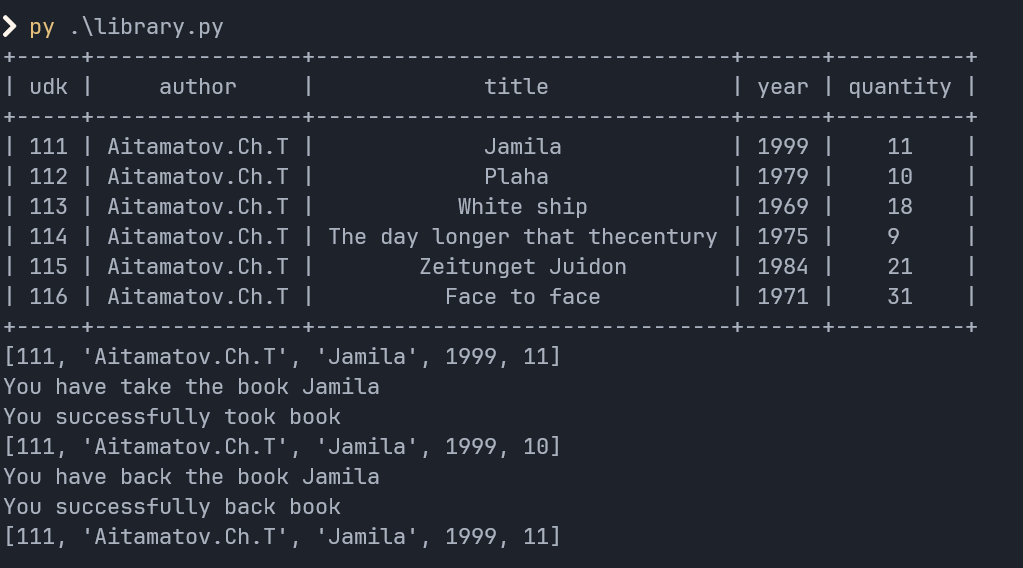
\includegraphics[width=0.8\textwidth]{./flowcharts/result_lib.png}
    \caption{Результат работы программы}
\end{figure}










\newpage
\section{Задача 2}

\subsection{Представления графа}

Необходимо представить граф:

\begin{figure}[H]
    \centering
    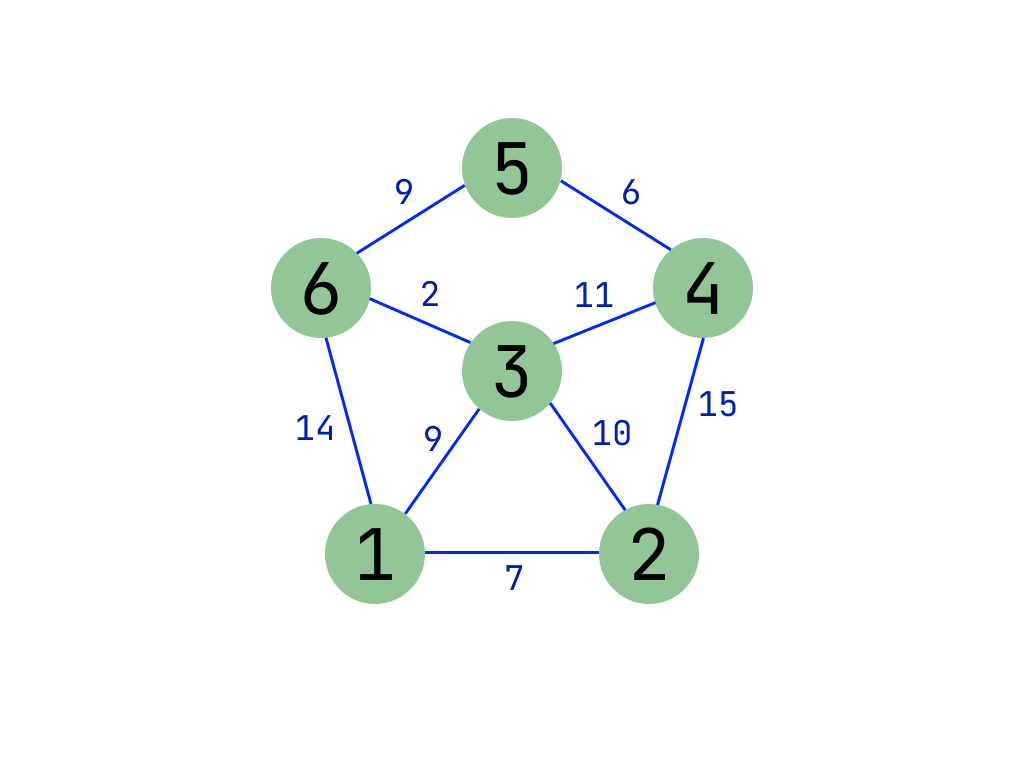
\includegraphics[width=0.8\textwidth]{./flowcharts/graph.png}
    \caption{Граф}
\end{figure}



Все четыре четыре способа способа представления 
графа можно реализовать на любом языке программирования 
используя 2-х или 3-х мерные массивы.


\begin{table}[!ht]
    \centering
    \caption{Матрица смежности}
    \begin{tabular}{|c|c|c|c|c|c|c|}
    \hline
        № & 1 & 2 & 3 & 4 & 5 & 6 \\ \hline
        1 & 0 & 7 & 9 & 0 & 0 & 14 \\ \hline
        2 & 7 & 0 & 10 & 15 & 0 & 0 \\ \hline
        3 & 9 & 10 & 0 & 11 & 0 & 2 \\ \hline
        4 & 0 & 15 & 11 & 0 & 6 & 0 \\ \hline
        5 & 0 & 0 & 0 & 6 & 0 & 9 \\ \hline
        6 & 14 & 0 & 2 & 0 & 9 & 0 \\ \hline
    \end{tabular}
    \label{Матрица смежности}
\end{table}



\begin{table}[!ht]
    \centering
    \caption{Матрица инцидентности}
    \begin{tabular}{|c|c|c|c|c|c|c|c|c|c|c|}
    \hline
        № & 1-2 & 1-3 & 1-6 & 2-3 & 2-4 & 3-4 & 3-5 & 3-6 & 4-5 & 5-6 \\ \hline
        1 & 1 & 1 & 1 & 0 & 0 & 0 & 0 & 0 & 0 & 0 \\ \hline
        2 & 1 & 0 & 0 & 1 & 1 & 0 & 0 & 0 & 0 & 0 \\ \hline
        3 & 0 & 1 & 0 & 1 & 0 & 1 & 0 & 1 & 0 & 0 \\ \hline
        4 & 0 & 0 & 0 & 0 & 1 & 1 & 0 & 0 & 1 & 0 \\ \hline
        5 & 0 & 0 & 0 & 0 & 0 & 0 & 1 & 0 & 1 & 1 \\ \hline
        0 & 0 & 1 & 0 & 0 & 0 & 0 & 0 & 1 & 0 & 1 \\ \hline
    \end{tabular}
    \label{Матрица инцидентности}
\end{table}



\begin{table}[!ht]
    \centering
    \caption{Списки смежности}
    \begin{tabular}{|c|c|}
    \hline
        Номер вершины & Смежные вершины \\ \hline
        1 & 2, 3, 6 \\ \hline
        2 & 1, 3, 4 \\ \hline
        3 & 1, 2, 4, 5 \\ \hline
        4 & 2, 3, 5 \\ \hline
        5 & 3, 4, 5 \\ \hline
        6 & 1, 3, 5 \\ \hline
    \end{tabular}
    \label{Списки смежности}
\end{table}



\begin{table}[!ht]
    \centering
    \caption{Списки рёбер}
    \begin{tabular}{|c|c|}
    \hline
        Номер ребра & Вершины, соединенные этим ребром \\ \hline
        1 & 1, 6 \\ \hline
        2 & 1, 3 \\ \hline
        3 & 1, 2 \\ \hline
        4 & 2, 3 \\ \hline
        5 & 2, 4 \\ \hline
        6 & 3, 4 \\ \hline
        7 & 3, 6 \\ \hline
        8 & 4, 5 \\ \hline
        9 & 5, 6 \\ \hline
    \end{tabular}
    \label{Списки рёбер}
\end{table}



\subsection{Алгоритм дейкстры}

\textbf{Словестное описание алгоритма: }

В простейшей реализации для хранения чисел \textit{d[i]} можно использовать массив чисел, а для хранения принадлежности элемента множеству U — массив булевых переменных.

В начале алгоритма расстояние для начальной вершины полагается равным нулю, а все остальные расстояния заполняются большим положительным числом (бо́льшим максимального возможного пути в графе). Массив флагов заполняется нулями. Затем запускается основной цикл.

На каждом шаге цикла мы ищем вершину $v$ с минимальным расстоянием и флагом равным нулю. Затем мы устанавливаем в ней флаг в 1 и проверяем все соседние с ней вершины $u$ Если в них (в $u$) расстояние больше, чем сумма расстояния до текущей вершины и длины ребра, то уменьшаем его. Цикл завершается, когда флаги всех вершин становятся равны 1, либо когда у всех вершин c флагом 0 $d[i]=\infty$. Последний случай возможен тогда и только тогда, когда граф G несвязный. 

\textbf{Блок схема алгоритма дейкстры}


\begin{figure}[H]
    \centering
    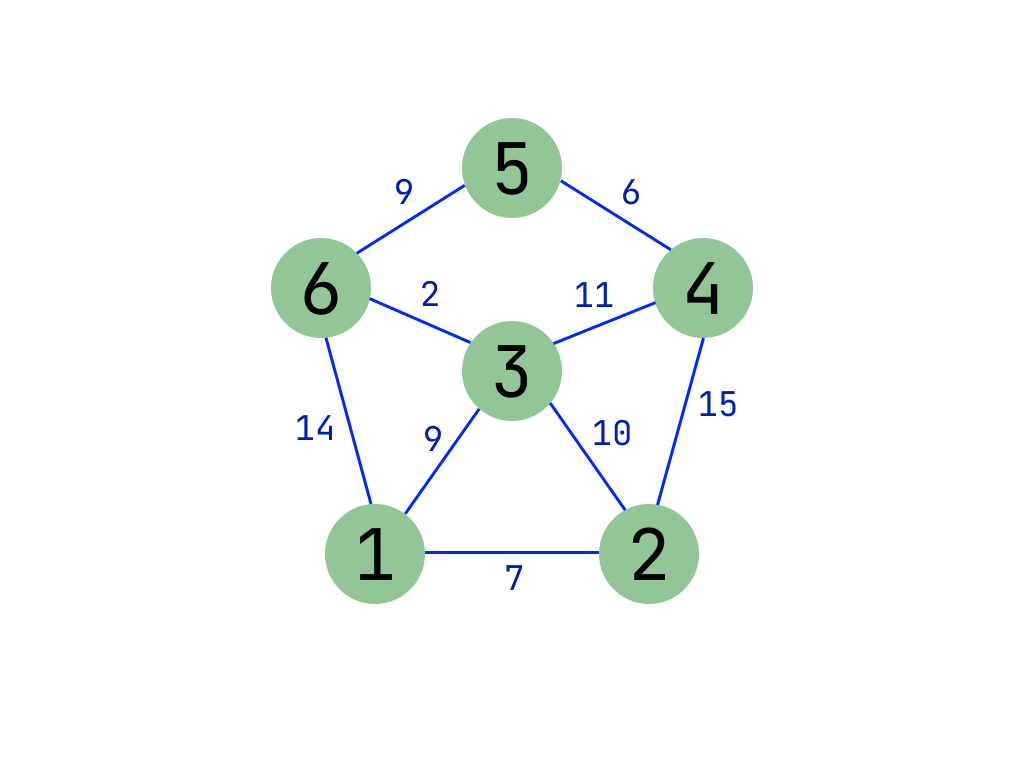
\includegraphics[width=0.8\textwidth]{./flowcharts/graph.png}
    \caption{Блок схема алгоритм Дейкстры}
\end{figure}


\textbf{Реализация на языке python}


\lstinputlisting[language = python]{../dijkstra.py}



\textbf{Результат выполнения программы}

\begin{figure}[H]
    \centering
    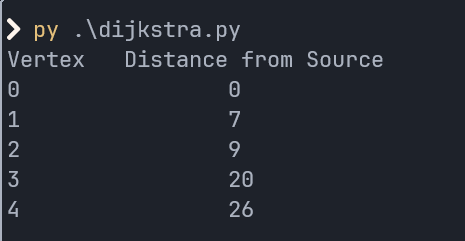
\includegraphics[width=0.8\textwidth]{./flowcharts/result.png}
    \caption{Результат работы программы}
\end{figure}


\textbf{Комплексность}

Комплексность данного алгоритма $O(N^2)$


\section{Ссылки}
Ссылка на весь код представленный в этом документе, а также исходный код самого документа вы можете найти по этой ссылке

\href{https://github.com/orenvadi/LAB3}{https://github.com/orenvadi/LAB3}



\end{document}
